\section{Model Assumptions}
    \begin{enumerate}
        \item The airflow entering the channel is turbulent. The Reynolds number exceeds 2300 at an inlet velocity ($U_{in}$) of 0.3 m/s.
        \item Portions of the fuel cell not part of the cathode flow field are impermeable to air. While carbon paper is porous, the in-plane pressure drop is much greater than that of the cathode flow field.
        \item The cathode flow field channels are modeled with a uniform height. The average offset (0.025 mm) is negligible compared to the channel height (1 mm).
        \item Cathode flow fields are modeled with straight edges and right-angle folds. The fold radius (0.05 mm) is small compared to the channel width (1 mm).
        \item Conservation of mass and momentum of airflow is assumed to be valid when transitioning between open spaces and cathode channels.
        \item A representative unit cell approximates the entire stack, excluding edge effects near the terminals. Airflow entering the unit cell is uniform and symmetrical.
        \item Channels are identical throughout the stack, resulting in no pressure drop differences between channels.
        \item The channels are fully dry without condensation. The oxidant stoichiometry exceeds 100, ensuring water vapor produced is absorbed by the airflow, negating the need for accounting water saturation.
        \item The losses from the fuel cell operation are converted to heat. 
    \end{enumerate}

    \section{Workflow - Pressure Drop}
    The following steps outline the workflow process for the unit cell simulations conducted in COMSOL:

    \begin{enumerate}
        \item \textbf{Selection of Laminar Flow Model:}
        \begin{itemize}
            \item This model was chosen because the airflow within the channels is laminar and is the largest contributor to the pressure drop across the stack.
            \item The laminar flow model allows for faster convergence and has been shown to be accurate when compared with experimental results.
        \end{itemize}
        
        \item \textbf{Construction of Unit Cell:}
        \begin{itemize}
            \item The unit cell was constructed using blocks with dimensions defined by equations to accommodate dimensional changes in the channels.
        \end{itemize}
        
        \item \textbf{Meshing Strategy:}
        \begin{itemize}
            \item A custom mesh was employed, focusing on the transition areas between inflow and outflow within the channels with a finer mesh.
            \item A coarser mesh was used within the channel and the air space between inflow and outflow.
            \item A mesh independence study was performed during the mesh fine-tuning. The results are shown in Figure ?.
            \item The difference between the blue dash (custom meshing) and green dots (physics-based extra fine meshing) is less than 3\%, thus the blue dash mesh was selected for its speed and accuracy.
        \end{itemize}
        
        \item \textbf{Parameter Sweep Function:}
        \begin{itemize}
            \item The parameter sweep function was utilized to explore all possible combinations for each stack size.
        \end{itemize}
        
        \item \textbf{Exporting Simulation Data:}
        \begin{itemize}
            \item The inputs and outputs of the simulations were exported from COMSOL for further analysis.
        \end{itemize}
    \end{enumerate}

    \section{Workflow - Temperature Stack}
    The following steps outline the workflow process for the unit cell simulations conducted in COMSOL:

    \begin{enumerate}
        \item \textbf{Selection of Physics Models:}
        \begin{itemize}
            \item The unit cell simulations were done using laminar flow physics as well as heat transfer in laminar flow.
            \item The parameter sweep function was utilized to explore all possible combinations in the parameter space.
            \item This model was selected because the flow through the channel is laminar and the simulation focuses on heat transfer within the channels.
        \end{itemize}
        
        \item \textbf{Construction of Unit Cell:}
        \begin{itemize}
            \item The unit cell was constructed using blocks with dimensions defined by equations to accommodate dimensional changes in the channels.
        \end{itemize}
        
        \item \textbf{Heat Generation Simulation:}
        \begin{itemize}
            \item Heat generation was simulated as a boundary heat source placed at the cathode side of the membrane.
        \end{itemize}
        
        \item \textbf{Heat Conduction Values:}
        \begin{itemize}
            \item The heat conduction values for each layer in the fuel cell were obtained from various papers, as shown in Table 8-1.
        \end{itemize}
        
        \item \textbf{Meshing Strategy:}
        \begin{itemize}
            \item A mesh independence study was conducted during the fine-tuning of the mesh. The results are shown in Figure ?.
            \item The difference between the blue dash and green dots is less than 1.06\%, hence the blue dash mesh was selected for its speed and accuracy.
        \end{itemize}
        
        \item \textbf{Exporting Simulation Data:}
        \begin{itemize}
            \item The inputs and outputs of the simulations were exported from COMSOL for further analysis.
        \end{itemize}
    \end{enumerate}

\newpage \section{Parameters}

    \begin{table}[h]
    \centering
    \begin{tabularx}{\textwidth}{X X X}
    \toprule
    \textbf{Name} & \textbf{Value} & \textbf{Unit} \\ 
    \midrule
    Cell Area & 0.005 & m$^2$ \\ 
    Cell Voltage & 0.6 & V \\ 
    Compression & 0.1 & - \\ 
    Current & 40 & A \\ 
    Hbp & 5$\times$10$^{-5}$ & m \\ 
    Hcc & 1.25$\times$10$^{-3}$ & m \\ 
    Hcp & 3.15$\times$10$^{-4}$ & m \\ 
    Hmem & 1.5$\times$10$^{-5}$ & m \\ 
    Kcp & 1.5 & W$\cdot$m$^{-1}$K$^{-1}$ \\ 
    Kmem & 0.1 & W$\cdot$m$^{-1}$K$^{-1}$ \\ 
    Lcc & 0.03 & m \\ 
    pRef & 1.0133$\times$10$^5$ & Pa \\ 
    Q & 5040 & W$\cdot$m$^{-2}$ \\ 
    Tamb & 293.15 & K \\ 
    Test & 25.2 & W \\ 
    Uin & 7.75 & m$\cdot$s$^{-1}$ \\ 
    Wcc & 0.001 & m \\ 
    Wr & 5$\times$10$^{-5}$ & m \\ 
    \bottomrule
    \end{tabularx}
    \caption{Parameter Values}
    \label{tab:parameters}
    \end{table}

\section{Materials}
    % Superscripts Table
    \begin{table}[H]
    \centering
    \begin{tabularx}{\textwidth}{BA}
    \toprule
    \textbf{Name} & \textbf{Unit} \\ 
    \midrule
    \multicolumn{2}{c}{\textbf{Air}} \\
    \midrule
    Dynamic viscosity & \( \text{Pa} \cdot \text{s} \) \\ 
    Ratio of specific heats & - \\ 
    Heat capacity at constant pressure & \(\text{J} / (\text{kg} \cdot \text{K})\) \\ 
    Density & \(\text{kg} / \text{m}^{3}\) \\ 
    Thermal conductivity & \(\text{W} / (\text{m} \cdot \text{K})\) \\
    \midrule
    \multicolumn{2}{c}{\textbf{Carbon Paper}} \\
    Density & \(\text{kg} / \text{m}^{3}\) \\ % No value
    Heat capacity at constant pressure & \(\text{J} / (\text{kg} \cdot \text{K})\) \\ % No value
    Thermal conductivity & \(\text{W} / (\text{m} \cdot \text{K})\) \\
    \midrule
    \midrule
    \multicolumn{2}{c}{\textbf{Membrane}} \\
    Thermal conductivity & \(\text{W} / (\text{m} \cdot \text{K})\) \\
    \midrule
    \midrule
    \multicolumn{2}{c}{\textbf{Steel Grade 316L}} \\
    Density & \(\text{kg} / \text{m}^{3}\) \\ % No value
    Heat capacity at constant pressure & \(\text{J} / (\text{kg} \cdot \text{K})\) \\ % No value
    Thermal conductivity & \(\text{W} / (\text{m} \cdot \text{K})\) \\
    \midrule
    \bottomrule
    \end{tabularx}
    \caption{Material Descriptions}
    \end{table}


\section{Laminar Flow}
    \subsection{Governing Equations}
        \begin{equation}
            \rho (\textbf{u} \cdot \nabla) \textbf{u} = \nabla \cdot \left[-p\textbf{I} + \textbf{K} \right] + \textbf{F} 
        \end{equation}
            \noindent where \(\rho\) is the density of air, \textbf{u} is the velocity vector, p is the pressure, \textbf{I} is the identity matrix, \textbf{K} is the viscous stress tensor, and \textbf{F} is the volume force vector.
        \begin{equation}
            \nabla \cdot (\rho \textbf{u})= 0 % The equation is different in the thesis
        \end{equation}
        \begin{equation}
            \textbf{K} = \mu (\nabla \textbf{u} + (\nabla \textbf{u})^T) - \frac{2}{3} \mu (\nabla \cdot \textbf{u})\textbf{I} % NOTE: The equation is different from the one in the thesis.
        \end{equation}
            where \textbf{\(\mu\)} is the dynamic viscosity of air. 

    \subsection{Initial Values}
        \begin{enumerate}
            \item Velocity field
                \begin{equation}
                    \textbf{u} = \textbf{0}
                \end{equation}
            \item Pressure
                \begin{equation}
                    p = 0
                \end{equation}
        \end{enumerate}

    \subsection{Boundary Conditions}
        \begin{enumerate}
            \item Wall (No slip)
                \begin{equation}
                    \mathbf{u} = \mathbf{0}
                \end{equation}
        
            \item Inlet (Velocity)
                \begin{equation}
                    \mathbf{u} = -U_{0} \mathbf{n}
                \end{equation}
                    where \(U_{0}\) is the initial velocity (i.e. normal inflow velocity) and \(\mathbf{n}\) is the unit normal vector. 
            
            \item Outlet (Pressure)
                \begin{equation}
                    \left[-p\textbf{I} + \textbf{K} \right]\mathbf{n} = - \hat{p}_{0} \mathbf{n} % this equation is different from the one in the thesis.
                \end{equation}
                \begin{equation}
                    \hat{p_{0}} \leq p_{0}, \nabla \mathbf{G} \cdot \mathbf{n} = 0
                \end{equation}
                    where \(\hat{p}_{0}\) is the estimated standard condition pressure, \(p_{0}=0\) is the standard condition pressure (i.e. suppress backflow), \(\mathbf{G}\) is the reciprocal wall distance. 
        
            \item Symmetry 
                \begin{equation}
                    \mathbf{u} \cdot \mathbf{n} = 0
                \end{equation}
                \begin{equation}
                    \mathbf{K}_{n} - (\mathbf{K}_{n} \cdot \mathbf{n})\mathbf{n} = 0, \mathbf{K}_{n} = \mathbf{Kn}
                \end{equation}
        \end{enumerate}
        
\section{Heat Transfer}
    \subsection{Governing Equations - Solid}
        \begin{equation}
            \rho C_{p} \textbf{u} \cdot \nabla T + \nabla \cdot \textbf{q} = Q + Q_{ted}
        \end{equation}
            \noindent where \(C_{p}\) is the specific heat capacity of air, T is the temperature of air, \textbf{q} is the heat flux vector, Q is the heat source, and \(Q_{ted}\) is the thermoelastic damping heat source.
        \begin{equation}
            \textbf{q} = -k \nabla T
        \end{equation}
            \noindent where k is the thermal conductivity. 
        \begin{equation}
            Q = (1.23 - Operating\ Voltage) \times \frac{Fuel\ Cell\ Stack\ Current}{Cell\ Area}
        \end{equation}
            
    \subsection{Governing Equations - Fluid}
        \begin{equation}
            \rho C_{p} \textbf{u} \cdot \nabla T + \nabla \cdot \textbf{q} = Q + Q_{p} + Q_{vd} % I dont know what vd is.
        \end{equation}
        \noindent where \(Q_{p}\) is the point heat source.
        \begin{equation}
            \textbf{q} = -k \nabla T
        \end{equation}
    
    \subsection{Governing Equations - Thin Layer}
        \begin{equation}
            -\textbf{n}_{d} \cdot \textbf{q}_{u} = \frac{(T_{u} - T_{d})}{R_{s}} + \frac{1}{2} d_{s} Q_{s}
        \end{equation}
        \noindent where \(R_s\) is the thermal resistance, and \(d_s\) is the thin layer thickness. 
        \begin{equation}
            -\textbf{n}_{u} \cdot \textbf{q}_{u} = \frac{(T_{d} - T_{u})}{R_{s}} + \frac{1}{2} d_{s} Q_{s}
        \end{equation}
        \begin{equation}
            R_{s} = \frac{d_{s}}{k_{s}}
        \end{equation}
    
    \subsection{Initial Values}
        \begin{enumerate}
            \item Temperature
                \begin{equation}
                    T = T_{amb}
                \end{equation}
                where \(T_{amb}\) is the initial ambient temperature.
        \end{enumerate}

    \subsection{Boundary Conditions}
        \begin{enumerate}
            \item Insulation
                \begin{equation}
                    -\mathbf{n} \cdot \mathbf{q} = 0
                \end{equation}
        
            \item Symmetry
                \begin{equation}
                    -\mathbf{n} \cdot \mathbf{q} = 0
                \end{equation}
        
            \item Boundary Heat Source
                \begin{equation}
                    -\mathbf{n} \cdot \mathbf{q} = Q_b
                \end{equation}
                where \(Q_b\) is the boundary heat source.
            
            \item Outflow
                \begin{equation}
                    -\mathbf{n} \cdot \mathbf{q} = 0
                \end{equation}
        
            \item Inlet
                \begin{equation}
                    T = T_{amb}
                \end{equation}
        \end{enumerate}

\section{Mesh}

\section{Study}
    \subsection{Difference between External and Internal Sweep}
        An internal sweep involves varying parameters directly within the 
        simulation model itself. This type of sweep is integrated into the 
        simulation process, where the solver automatically adjusts the parameters 
        as part of its internal algorithm. Internal sweeps are typically used to 
        explore the parameter space of the model in a more automated and 
        controlled manner, often leveraging the solver's built-in capabilities 
        to iterate through different parameter values.

        
        \vspace{1em} \noindent An external sweep, on the other hand, involves varying parameters outside 
        of the simulation model. This is usually managed by an external script 
        or control mechanism that systematically modifies the input parameters, 
        runs the simulation for each set of parameters, and collects the results. 
        External sweeps provide more flexibility and control over the parameter 
        variations and can be useful for complex scenarios where the internal 
        capabilities of the solver might be limited.
    \subsection{Parametric Sweep}
        A parametric sweep is a systematic method used in simulations and computational 
        experiments to explore the effects of varying parameters within a defined range. 
        By adjusting one or more input parameters incrementally, researchers can observe 
        how changes influence the outcome, enabling a comprehensive analysis of the 
        system's behavior. This technique is essential for optimizing designs, 
        identifying critical factors, and understanding the sensitivity of the results 
        to different variables. Ultimately, parametric sweeps provide valuable insights 
        that drive informed decision-making and innovation.

        \begin{table}[h]
        \centering
        \begin{tabularx}{\textwidth}{X X X}
        \toprule
        \textbf{Name} & \textbf{Values} & \textbf{Unit} \\ 
        \midrule
        Hcc & 1 1.25 1.5 1.75 2 & \(\text{mm}\) \\ 
        Wcc & 0.5 0.75 1 1.25 1.5 & \(\text{mm}\) \\ 
        Lcc & 30 60 90 & \(\text{mm}\) \\ 
        \bottomrule
        \end{tabularx}
        \caption{Parameter Sweep Values for All Combinations}
        \end{table}
    \subsection{Auxilary Sweep}
        An auxiliary sweep is a computational technique used to study the influence
        of secondary parameters or variables that are not directly part of the main 
        parametric study. It involves varying these auxiliary parameters to 
        investigate their impact on the primary simulation or experiment results. 
        This approach helps in understanding the interactions and dependencies 
        between primary and auxiliary parameters, providing a deeper insight into 
        the system's overall behavior. Auxiliary sweeps are particularly useful in 
        complex models where multiple factors may indirectly affect the outcomes, 
        aiding in fine-tuning and enhancing the accuracy of simulations.

        \begin{table}[h]
        \centering
        \begin{tabularx}{\textwidth}{X X X}
        \toprule
        \textbf{Name} & \textbf{Values} & \textbf{Unit} \\ 
        \midrule
        Uin & 1 3.25 5.5 7.75 10 & \(\text{m}/\text{s}\) \\ 
        Q & 1272 3132 5040 & \(W/\text{m}^{-2}\) \\ 
        Tamb & -20 0 20 40 & \(\degree \text{C}\) \\ 
        \bottomrule
        \end{tabularx}
        \caption{Auxilary Sweep Values for All Combinations}
        \end{table}
    
    \section{Results}
        \subsection{Accumulated Probe Table: Set 1}
            \begin{enumerate}
                \item Hcc (1 - hc)
                \item Wcc (2 - wc)
                \item Lcc (3 - length)
                \item Tamb (4 - Tamb)
                \item Q (5 - Q)
                \item Uin (6 - Uin)
                \item Delp (15 - Pressure (Pa), Pressure Probe 3)
                    \begin{figure}[H]
                        \centering
                        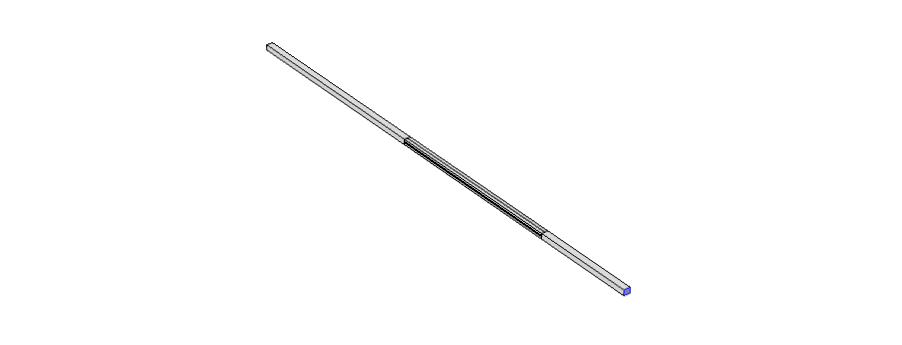
\includegraphics[width=1\textwidth]{00_Images/00_Pressure_Probe_3.png}
                        \caption{Pressure Probe 3 Location}
                    \end{figure}
                \item Tsta (18 - Temperature (degC), Stack Temperature Probe 1)
                    \begin{figure}[H]
                        \centering
                        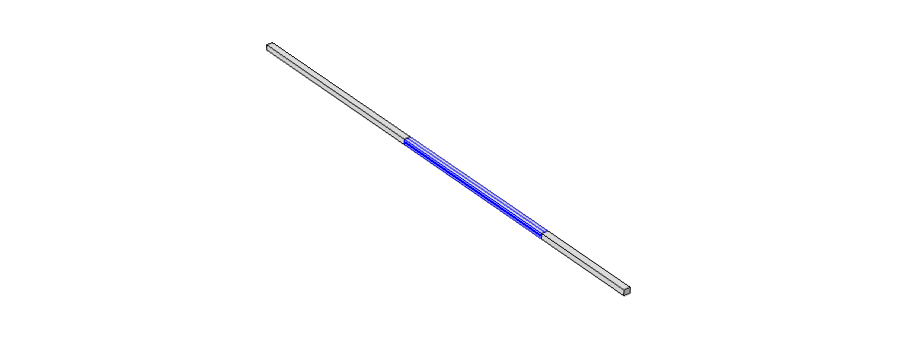
\includegraphics[width=1\textwidth]{00_Images/00_Stack_Temperature_Probe_1.png}
                        \caption{Stack Temperature Probe 1 Location}
                    \end{figure}
            \end{enumerate}

        \subsection{3D Plots}
            \begin{enumerate}
                \item Pressure Drop
                    \begin{figure}[H]
                        \centering
                        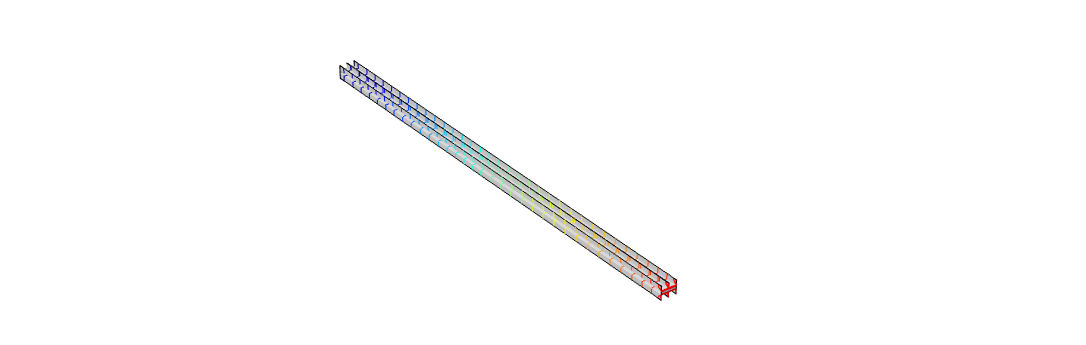
\includegraphics[width=1\textwidth]{00_Images/00_Pressure.png}
                        \caption{Pressure Drop 3D Plot}
                    \end{figure}
                \item Temperature Stack
                    \begin{figure}[H]
                        \centering
                        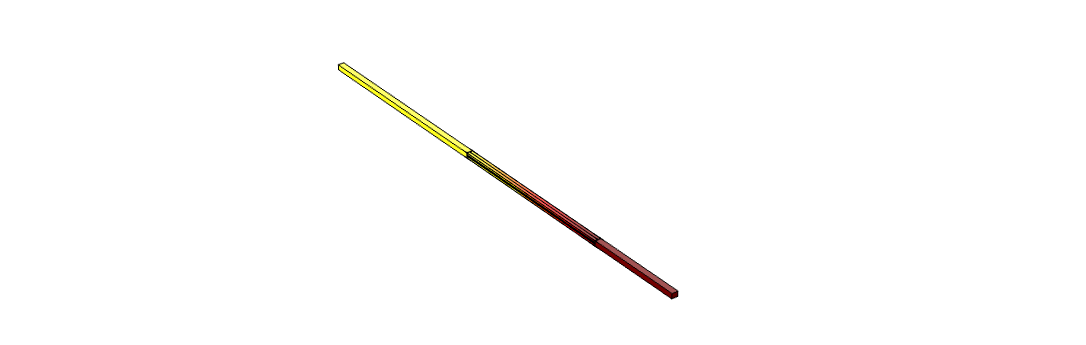
\includegraphics[width=1\textwidth]{00_Images/00_Temperature.png}
                        \caption{Temperature Stack 3D Plot}
                    \end{figure}
                \item Velocity 
                    \begin{figure}
                        \centering
                        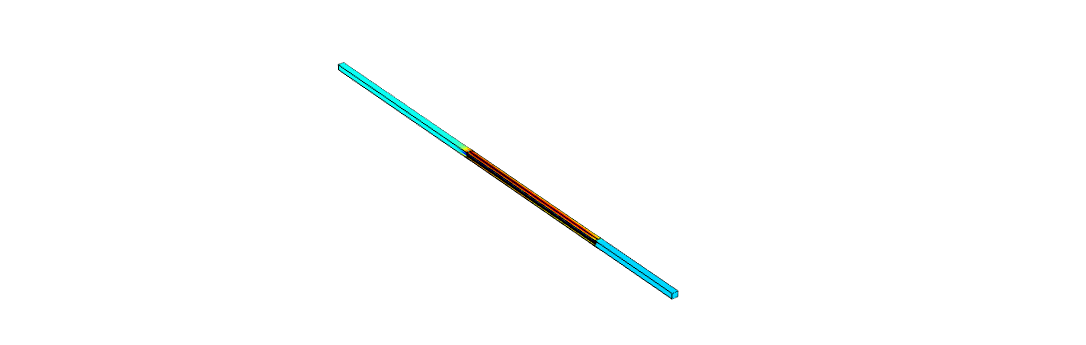
\includegraphics[width=1\textwidth]{00_Images/00_Velocity.png}
                        \caption{Velocity 3D Plot}
                    \end{figure}
            \end{enumerate}